%Version 3 October 2023
% See section 11 of the User Manual for version history
%
%%%%%%%%%%%%%%%%%%%%%%%%%%%%%%%%%%%%%%%%%%%%%%%%%%%%%%%%%%%%%%%%%%%%%%
%%                                                                 %%
%% Please do not use \input{...} to include other tex files.       %%
%% Submit your LaTeX manuscript as one .tex document.              %%
%%                                                                 %%
%% All additional figures and files should be attached             %%
%% separately and not embedded in the \TeX\ document itself.       %%
%%                                                                 %%
%%%%%%%%%%%%%%%%%%%%%%%%%%%%%%%%%%%%%%%%%%%%%%%%%%%%%%%%%%%%%%%%%%%%%

%%\documentclass[referee,sn-basic]{sn-jnl}% referee option is meant for double line spacing

%%=======================================================%%
%% to print line numbers in the margin use lineno option %%
%%=======================================================%%

%%\documentclass[lineno,sn-basic]{sn-jnl}% Basic Springer Nature Reference Style/Chemistry Reference Style

%%======================================================%%
%% to compile with pdflatex/xelatex use pdflatex option %%
%%======================================================%%

%%\documentclass[pdflatex,sn-basic]{sn-jnl}% Basic Springer Nature Reference Style/Chemistry Reference Style


%%Note: the following reference styles support Namedate and Numbered referencing. By default the style follows the most common style. To switch between the options you can add or remove �Numbered� in the optional parenthesis. 
%%The option is available for: sn-basic.bst, sn-vancouver.bst, sn-chicago.bst%  
 
%%\documentclass[sn-nature]{sn-jnl}% Style for submissions to Nature Portfolio journals
%%\documentclass[sn-basic]{sn-jnl}% Basic Springer Nature Reference Style/Chemistry Reference Style
\documentclass[sn-mathphys-num]{sn-jnl}% Math and Physical Sciences Numbered Reference Style 
%%\documentclass[sn-mathphys-ay]{sn-jnl}% Math and Physical Sciences Author Year Reference Style
%%\documentclass[sn-aps]{sn-jnl}% American Physical Society (APS) Reference Style
%%\documentclass[sn-vancouver,Numbered]{sn-jnl}% Vancouver Reference Style
%%\documentclass[sn-apa]{sn-jnl}% APA Reference Style 
%%\documentclass[sn-chicago]{sn-jnl}% Chicago-based Humanities Reference Style

%%%% Standard Packages
%%<additional latex packages if required can be included here>
\usepackage[english]{babel}
\usepackage{graphicx}%
\usepackage{multirow}%
\usepackage{multicol}
\usepackage{amsmath,amssymb,amsfonts}%
\usepackage{amsthm}%
\usepackage{mathrsfs}%
\usepackage[title]{appendix}%
\usepackage{xcolor}%
\usepackage{textcomp}%
\usepackage{manyfoot}%
\usepackage{booktabs}%
\usepackage{algorithm}%
\usepackage{algorithmicx}%
\usepackage{algpseudocode}%
\usepackage{listings}%
\usepackage{siunitx}
\usepackage{refcheck}
\usepackage{threeparttable}
%\usepackage{array}
%\usepackage{tabularray}
\DeclareSIUnit\year{yr}
%%%%

%%%%%=============================================================================%%%%
%%%%  Remarks: This template is provided to aid authors with the preparation
%%%%  of original research articles intended for submission to journals published 
%%%%  by Springer Nature. The guidance has been prepared in partnership with 
%%%%  production teams to conform to Springer Nature technical requirements. 
%%%%  Editorial and presentation requirements differ among journal portfolios and 
%%%%  research disciplines. You may find sections in this template are irrelevant 
%%%%  to your work and are empowered to omit any such section if allowed by the 
%%%%  journal you intend to submit to. The submission guidelines and policies 
%%%%  of the journal take precedence. A detailed User Manual is available in the 
%%%%  template package for technical guidance.
%%%%%=============================================================================%%%%

%% as per the requirement new theorem styles can be included as shown below
\theoremstyle{thmstyleone}%
\newtheorem{theorem}{Theorem}%  meant for continuous numbers
%%\newtheorem{theorem}{Theorem}[section]% meant for sectionwise numbers
%% optional argument [theorem] produces theorem numbering sequence instead of independent numbers for Proposition
\newtheorem{proposition}[theorem]{Proposition}% 
%%\newtheorem{proposition}{Proposition}% to get separate numbers for theorem and proposition etc.

\theoremstyle{thmstyletwo}%
\newtheorem{example}{Example}%
\newtheorem{remark}{Remark}%

\theoremstyle{thmstylethree}%
\newtheorem{definition}{Definition}%

\raggedbottom
%%\unnumbered% uncomment this for unnumbered level heads

\begin{document}

\title[GWRecharge]{Estimating groundwater recharge using a GIS-based distributed water balance model in Jordan River Watershed, Colombia}

%%=============================================================%%
%% GivenName	-> \fnm{Joergen W.}
%% Particle	-> \spfx{van der} -> surname prefix
%% FamilyName	-> \sur{Ploeg}
%% Suffix	-> \sfx{IV}
%% \author*[1,2]{\fnm{Joergen W.} \spfx{van der} \sur{Ploeg} 
%%  \sfx{IV}}\email{iauthor@gmail.com}
%%=============================================================%%

\author*[1]{\fnm{Oscar} \sur{Garc\'ia-Cabrejo}}\email{oscar.garcia04@uptc.edu.co}

%\author[2,3]{\fnm{Second} \sur{Author}}\email{iiauthor@gmail.com}
%\equalcont{These authors contributed equally to this work.}

%\author[1,2]{\fnm{Third} \sur{Author}}\email{iiiauthor@gmail.com}
%\equalcont{These authors contributed equally to this work.}

\affil*[1]{\orgdiv{Escuela de Ingenier\'ia Geol\'ogica}, \orgname{Universidad Pedag\'ogica y Tecnol\'ogica de Colombia}, \orgaddress{\street{ Calle 4 A Sur No. 15-13}, \city{Sogamoso}, \postcode{100190}, \state{Boyac\'a}, \country{Colombia}}}

%\affil[2]{\orgdiv{Department}, \orgname{Organization}, \orgaddress{\street{Street}, \city{City}, \postcode{10587}, \state{State}, \country{Country}}}

%\affil[3]{\orgdiv{Department}, \orgname{Organization}, \orgaddress{\street{Street}, \city{City}, \postcode{610101}, \state{State}, \country{Country}}}

%%==================================%%
%% Sample for unstructured abstract %%
%%==================================%%

%\abstract{The abstract serves both as a general introduction to the topic and as a brief, non-technical summary of the main results and their implications. Authors are advised to check the author instructions for the journal they are submitting to for word limits and if structural elements like subheadings, citations, or equations are permitted.}

%%================================%%
%% Sample for structured abstract %%
%%================================%%
%This derivation requires an assumption on the probability distribution of the number of traces types where trinomial and Poisson distributions are considered.
%The methodology is applied in three cases (two synthetic and a real case). The results show that the confidence regions of the trace parameters defined by the two previously mentioned approaches are similar with a high degree of overlap specially in the case of large number of traces.
% define the input parameters for discrete fracture network models, define ranges of rock mass indices and/or compare exposures at several locations. 
 \abstract{
 %\textbf{Background:57} 
 Groundwater management requires a proper characterization of the spatial and temporal variation of the groundwater recharge. GIS-based methods have become a viable alternative for groundwater recharge estimation. 
 %\textbf{Problem:23} 
 This is specially important in data-scarce regions such as the Jordan River Watershed in Colombia where no groundwater monitoring network, shallow aquifers and incipient use of groundwater.  
 %\textbf{Methods:76} 
In this study, the groundwater recharge is estimated using a GIS-based soil water balance model that considers the spatial variation in the topography, soil and hydrological properties in the study area for different water years.
 %\textbf{Results:68} 
 The spatial and long-term average of the annual rainfall of \SI{702}{\milli \meter} in a normal year is distributed as: surface runoff of \SI{292.4}{\milli \meter} (41.64\%), actual evapotranspiration of \SI{408.4}{\milli \meter} (52.8\%) and recharge of \SI{6.4}{\milli \meter} (0.9\%). The spatial and long-term average of the annual rainfall reduces to \SI{490}{\milli \meter} in dry years and increases to \SI{900}{\milli \meter} in wet years. The percentages of the surface runoff and actual evapotranspiration do not change according to the water years, whereas the recharge reduces to \SI{0.0}{\milli \meter} in dry years and \SI{33.4}{\milli \meter} (3.6\%) during wet years.
 %\textbf{Conclusion:22} 
 These recharge estimates corresponds to \SI{64.5}{\litre \per \second} during a normal year that increases to \SI{337}{\litre \per \second} during a wet year for a \SI{318.2}{\kilo \meter \squared} watershed. Therefore, the spatial and temporal variation of groundwater recharge should be considered in the formulation of a sustainable groundwater resources management plan for the Jordan River watershed. 
 }

\keywords{Aquifer recharge, GIS, Water balance model, Jordan River, Colombia}

%%\pacs[JEL Classification]{D8, H51}

%%\pacs[MSC Classification]{35A01, 65L10, 65L12, 65L20, 65L70}

\section*{Highlights}
\begin{itemize}
	\item H1
	\item  H2
	\item H3
	\item H4  
\end{itemize}


\maketitle

\section{Introduction}\label{sect:intro}

%The Introduction section, of referenced text \cite{bib1} expands on the background of the work (some overlap with the Abstract is acceptable). The introduction should not include subheadings.
%
%Springer Nature does not impose a strict layout as standard however authors are advised to check the individual requirements for the journal they are planning to submit to as there may be journal-level preferences. When preparing your text please also be aware that some stylistic choices are not supported in full text XML (publication version), including coloured font. These will not be replicated in the typeset article if it is accepted. 

\begin{itemize}
	\item \textbf{Introduce the topic} 
	\item \textbf{What has been done}
	\begin{itemize}
		\item \cite{Binder1997} water balance.
		\item \cite{healy2010}
		\item \cite{Galvao2018}
		\item \cite{Caro2023}
		\item GW in Colombia \cite{Loboguerrero1987,ArangurenDiaz2024}
	\end{itemize} 
	\item \textbf{Identify the GAP} 
	\item \textbf{Introduce your work} 
	\item \textbf{Research Questions}
	\begin{itemize}
		\item Q1: What is the magnitude of annual and monthly GW recharge in Tunja for normal, dry and wet years?
		\item Q2: Where are the places where the GW Recharge is high/low for normal, dry and wet years? Are these places consistent with the recharge zones identified in previous studies?
		\item Q3: What are the months when the GW Recharge is high/low during the normal, dry and wet years?
	\end{itemize}
\end{itemize}

\section{Study Area}

The Jordan River Watershed is situated in central Boyaca Department, Colombia, approximately \SI{130}{\kilo \meter} northeast of Bogota (between [longitude range] and [latitude range]). Encompassing an area of \SI{318.2}{\kilo \meter \squared}, the watershed is drained by the Vega River, the region's primary surface water source, which flows from southwest (SW) to northeast (NE).\\
\ \\
Key municipalities within the watershed include Tuta, Combita, Oicata, Chivata, Motavita, and Tunja (the state capital; see Fig.\ref{fig:location}). The area supports an estimated population of 200,000, with Tunja accounting for roughly 180,000 residents. Economically, the region relies predominantly on agriculture with limited industrial activity.\\
\ \\
While surface water (rivers, creeks, and springs) remains the principal water source, groundwater extraction has grown increasingly critical for human consumption and economic activities due to declining surface water availability. The terrain exhibits elevations ranging from \qtyrange{2546}{3312}{\meter} above sea level (masl), characterized by valleys, hills, and mountains typical of the Andean cordillera.\\
\ \\
The mean temperature over this area is \SI{13}{\degreeCelsius}. There are two rainy seasons distributed over the year, from March to May and from September to November, respectively. The  annual total precipitation ranges between NUMBERS. The climate in the area is classified as subtropical highland climate (Koppen Cfb), a type of climate characterized by mild temperatures and significant seasonal rainfall differences. This climate is typically found in mountainous or elevated regions within the tropics or subtropics. It's known for mild winters, especially in the subtropics, and wet summers.\\
\ \\
The geological evolution of the Jordan River Watershed began during the Upper Cretaceous with the deposition of marine sediments from the Guadalupe Group, comprising the Plaeners Formation (siliceous claystones) and the Labor y Tierna Formation (coarse-grained sandstones). From the Upper Maastrichtian to Upper Paleocene, deltaic and fluvial environments deposited shales and silty sandstones of the Guaduas Formation. Subsequently, during the Upper Paleocene to Lower Eocene, the Bogota Formation accumulated, characterized by fluvial-origin shales and siltstones interbedded with sandstone layers. In the Pliocene, fluvial and lacustrine systems deposited the coarse to very coarse conglomerates and sandstones of the Tilata Formation. During the Quaternary, alluvial sedimentation associated with the Jordan River's activity started and persists to the present day. \textbf{ADD GEOLOGICAL SYMBOLS AND REFERENCES}.\\
\ \\
The study area lies within Colombia's Eastern Cordillera which is characterized by a dominant northeast (NE) structural trend. This orientation aligns with the predominant direction of folds and faults in the region. The principal geological structures include the Tunja Syncline, along with the Arcabuco and Toca Anticlines. \textbf{ADD REFERENCES}\\
\ \\
The main aquifers in the study area consist of the Bogota Formation in the southwestern (SW) sector near Tunja, and both the Bogota and Tilata Formations in the northeastern (NE) sector. The Bogota Formation lies along the western flank of the Tunja Syncline, forming a closed aquifer system due to the absence of a clear discharge zone. In contrast, the Tilata Formation is primarily situated near the hinge of the syncline, with its discharge area located in the northeastern portion of the JRW.\\
\ \\
The city of Tunja has $12$ active wells, averaging \SI{200}{\meter} in depth, which supply water for human consumption via the municipal aqueduct (Veolia Corporation). These wells extract groundwater from the Bogota and Tilata formations. The Bogota Formation exhibits transmissivity values ranging from \qtyrange{5}{162}{\meter \squared \per \day}, varying with layer thickness. However, reliable storage coefficient estimates are unavailable due to pumping tests conducted without observation wells.\\
\ \\
A significant decline in hydraulic heads has been observed in the Bogota and Tilata Formation aquifers (USTA, 2015; others), reflecting intensive groundwater use and inadequate resource management. In the study area, estimated groundwater withdrawals total \SI{1.55e6}{\cubic \meter \per \year} (\SI{49}{\liter \per \second}) (USTA, 2015).

\begin{figure}
	\centering
	\includegraphics[scale=0.5]{location_optimized.pdf}
	\caption{Location of the Jordan River Watershed, Boyaca State, Colombia.}\label{fig:location}
\end{figure}



\section{Methodology}

The methodology used to estimate the GWR is based on a GIS-based soil water budget proposed by \cite{Galvao2018} that extended the methods developed by  \cite{Fenn1975} and OTHERS. This approach is composed of two stages calculation of runoff coefficients and Soil Water Budget, which are presented in Figure \ref{fig:methodology} and described below.

\begin{figure}
	\centering
	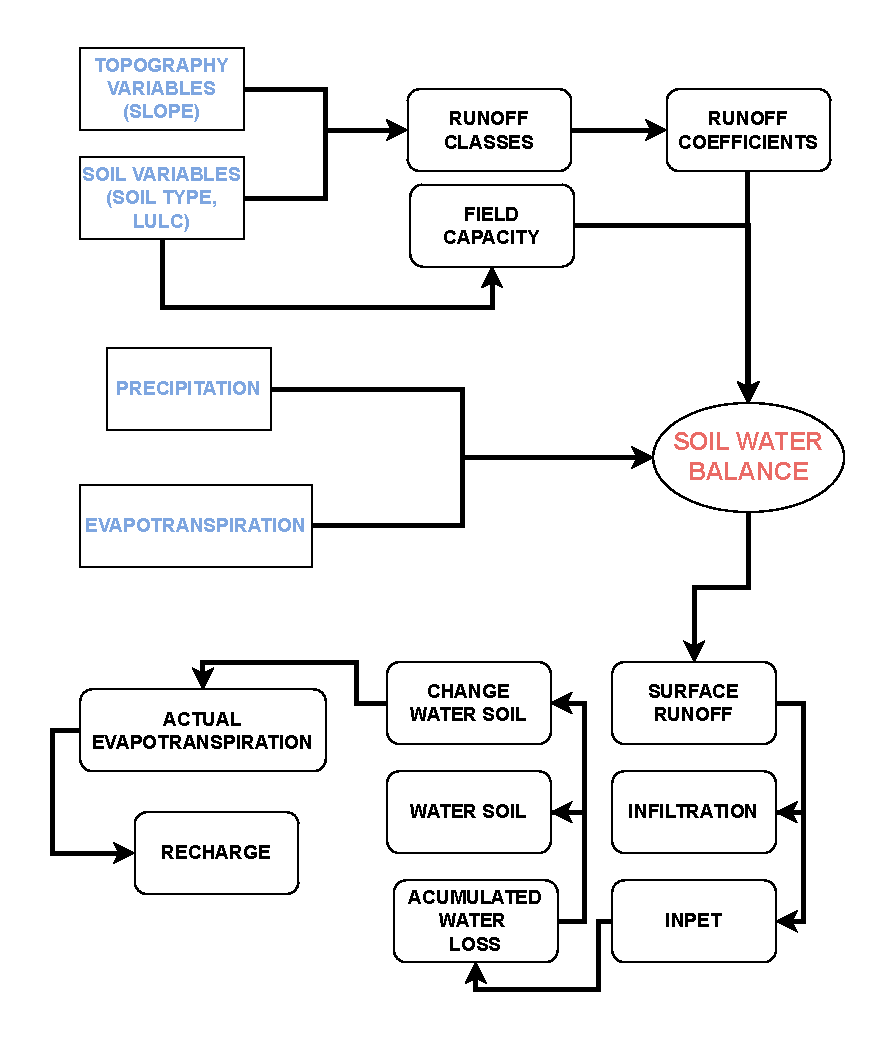
\includegraphics[scale=0.6]{methodology.pdf}
	\caption{Flowchart of the methodology followed in this work. The input variables are shown in blue whereas the calculated variables are shown in black. }\label{fig:methodology}
\end{figure}
%%%%%%%%%%%%%%%%%%%%%%%%%%%%%%%%%%%%%
\subsection{Runoff Coefficients}
The runoff coefficients are calculated for the entire watershed using information from soil permeability, infiltration capacity and slope. The soil permeability is defined from the content of clay/silt/sand of the soil. Soils with high content of sand are considered as permeable whereas the soils with high clay/silt content are considered impermeable. Soils with high permeability and low runoff are considered as favorable for GWR. The infiltration capacity is defined from the land cover, where forest/savannah and anthropic/grassy uses  are associated with high and low infiltration capacity, respectively. The GWR occurs mainly in areas with forest/savannah uses. The slope map is reclassified in three different intervals: low slopes $<2\%$, moderate slopes $2-7\%$ and steep slopes $>7\%$. The GWR is associated with low slopes where the water can easily infiltrate. A total of $12$ runoff classes are defined by the  combination of the soil permeability (2 classes), infiltration capacity (2 classes) and slope (3 classes). Runoff coefficients are assigned to each one of these classes using the tabulated values in \cite{ASCE1969}.  

All calculations are done in rasters.
Reference to Tables for soil permeability, infiltration capacity, slope. 

\begin{table}[h]
	\centering
	\begin{tabular}{ccccc} \hline
		\textbf{Soil Permeability} & \textbf{Infiltration Capacity} & \textbf{Terrain Slope} & \textbf{Classification} & \textbf{Runoff Coefficient} \\ \hline
		\multirow{6}{*}{Sandy} & Forest & $<2$ & Class 1 & $0.1$ \\
		&Savannah & $2-7$ & Class 2 & $0.1$ \\ 
		&&$>7$ &Class 3 & $0.3$ \\
		&Anthropic & $<2$ & Class 4 & $0.2$ \\ 
		&Grassy & $2-7$ & Class 5 & $0.3$ \\ 
		&&$>7$ &Class 6 & $0.4$ \\ \hline
		\multirow{6}{*}{Silty} & Forest & $<2$ & Class 7 & $0.3$\\
		&Savannah & $2-7$ & Class 8 & $0.4$ \\ 
		&&$>7$ &Class 9 & $0.5$ \\
		&Anthropic & $<2$ & Class 10 & $0.4$ \\ 
		&Grassy & $2-7$ & Class 11 & $0.5$ \\ 
		&&$>7$ &Class 12 & $0.6$\\ \hline
	\end{tabular}
	\caption{Classification criteria for the soil and topographical information according to \cite{ASCE1969} and \citep{Galvao2018}. EXPLANATION. Low runnoff coefficients are associated with permeable soils (sand), high infiltration capacity (forest areas) and small slopes (flat regions), areas that favor the recharge process. In contrast high runoff coefficients are related to impermeable soils (clay), low infiltration capacity (Grass areas) and high slopes (mountains), which represents unfavorable conditions for groundwater recharge. }\label{tab:runoff_classes}
\end{table}

%%%%%%%%%%%%%%%%%%%%%%%%%%%%%%%%%%%%%
\subsection{Soil Water Balance}
In this stage, the annual soil water budget is calculated using the approach proposed by \cite{Thornthwaite1955}.  This method only requires monthly averages of precipitation and evapotranspiration.  The soil water balance for a raster cell at a given month $i$ is given by:
\begin{equation}
P_{i}=R_{i}+AET_{i}+CWS_{i}+REC_{i}
\end{equation}
where
\begin{itemize}
\item $P_{i}$ is the precipitation 
\item $AET_{i}$ is the actual evapotranspiration
\item $CWS_{i}$ is the change in the water stored in the soil
\item $REC_{i}$ is the recharge
\end{itemize}
The surface runoff is calculated using the rational approach as the product of the runoff coefficients and the precipitation:
\begin{equation}
R_{i}=RC \times P_{i}
\end{equation}
where $RC$ is the runoff coefficient which depends on the soil type and use, and slope. 

The infiltration is the difference between the precipitation and the surface runoff:
\begin{equation}
IN_{i}=P_{i}-R_{i}
\end{equation}

The difference between infiltration and potential evapotranspiration is called IN-PET
\begin{equation}
INPET_{i}=IN_{i}-PET_{i}
\end{equation}
A positive INPET indicates a potential accumulation of water in the soil, whereas  the soil is drying if the INPET is negative. 

The accumulated water loss is the sum of the negative values of the INPET since the beginning of the year:
\begin{equation}
AWL_{i}=\sum\limits_{j=0}^{i}\text{NEG}(INPET_{j})
\end{equation}
The water stored in the soil can be calculated as follows:
\begin{equation}
WS_{i}=\left\{
\begin{aligned}
	&FC \times 10^{(b \times INPET_{i})} &\text{If } INPET_{i} < 0 \\
	&WS_{i-1} & \text{If } INPET_{i} > 0
\end{aligned}
\right.
\end{equation}
where
\begin{equation}
b=\frac{0.455}{FC}
\end{equation}
and $FC$ is the field capacity.\\
\ \\
The change in water storage is the difference between the water stored for a given month and the water stored in a previous month:
\begin{equation}
CWS_{i}=WS_{i}-WS_{i-1}
\end{equation}

There is actual evapotranspiration if  INPET is positive, that, is, the infiltration exceeds the potential evapotranspiration:
$$
AET_{i}=\left\{
\begin{aligned}
	&PET_{i} &\text{If } INPET_{i} \ge 0 \\
	&PET_{i}+[INPET_{i}-CWS_{i}] &\text{If } INPET_{i} < 0 \\
\end{aligned}
\right.
$$

The recharge can be calculate as follows:
$$
REC_{i}=\left\{
\begin{aligned}
	&INPET_{i}-CWS_{i} &\text{If } INPET_{i}>0\\
	&0 &\text{If } INPET_{i}<0\\
\end{aligned}
\right.
$$
\subsection{Input Data}

\subsubsection{Soil Information}

The soil map of study area was obtained from the Colombian Geographical Institute \cite{IGAC2005}  (see Figure \ref{fig:soil}a-b). The order of the soils present in the study area include Alfisols, Andisols, Entisols, Inceptisols, Mollisols, Miscelaneous and urban zones.  Inceptisols (sandy soils) are the most frequent type of soils located in the NE part of the study area and the NW and SE part of the Tunja municipality. Alfisols (silty soils) are the second most frequent type of soil located in several places across the study area (see pink color in Fig.  \ref{fig:soil}a).  The location of the sandy soils coincide with the inceptsoils previously described, whereas the impermeable silty soils are mainly located in the central part of the study area as shown in green colors in Figure  \ref{fig:soil}b.\\
\ \\
The land cover map of the study area is base on information provided by the Colombian Geographical Institute  \cite{IGAC2005} (see Figure \ref{fig:soil}c). Most of the area has agriculture/pastureland use and in minor proportion forests. The soil use reclassified is shown in Figure \ref{fig:soil}d which indicates that PERCENTAGE AREA of the study area is composed of materials with low infiltration capacity.

\begin{figure}
	\centering
	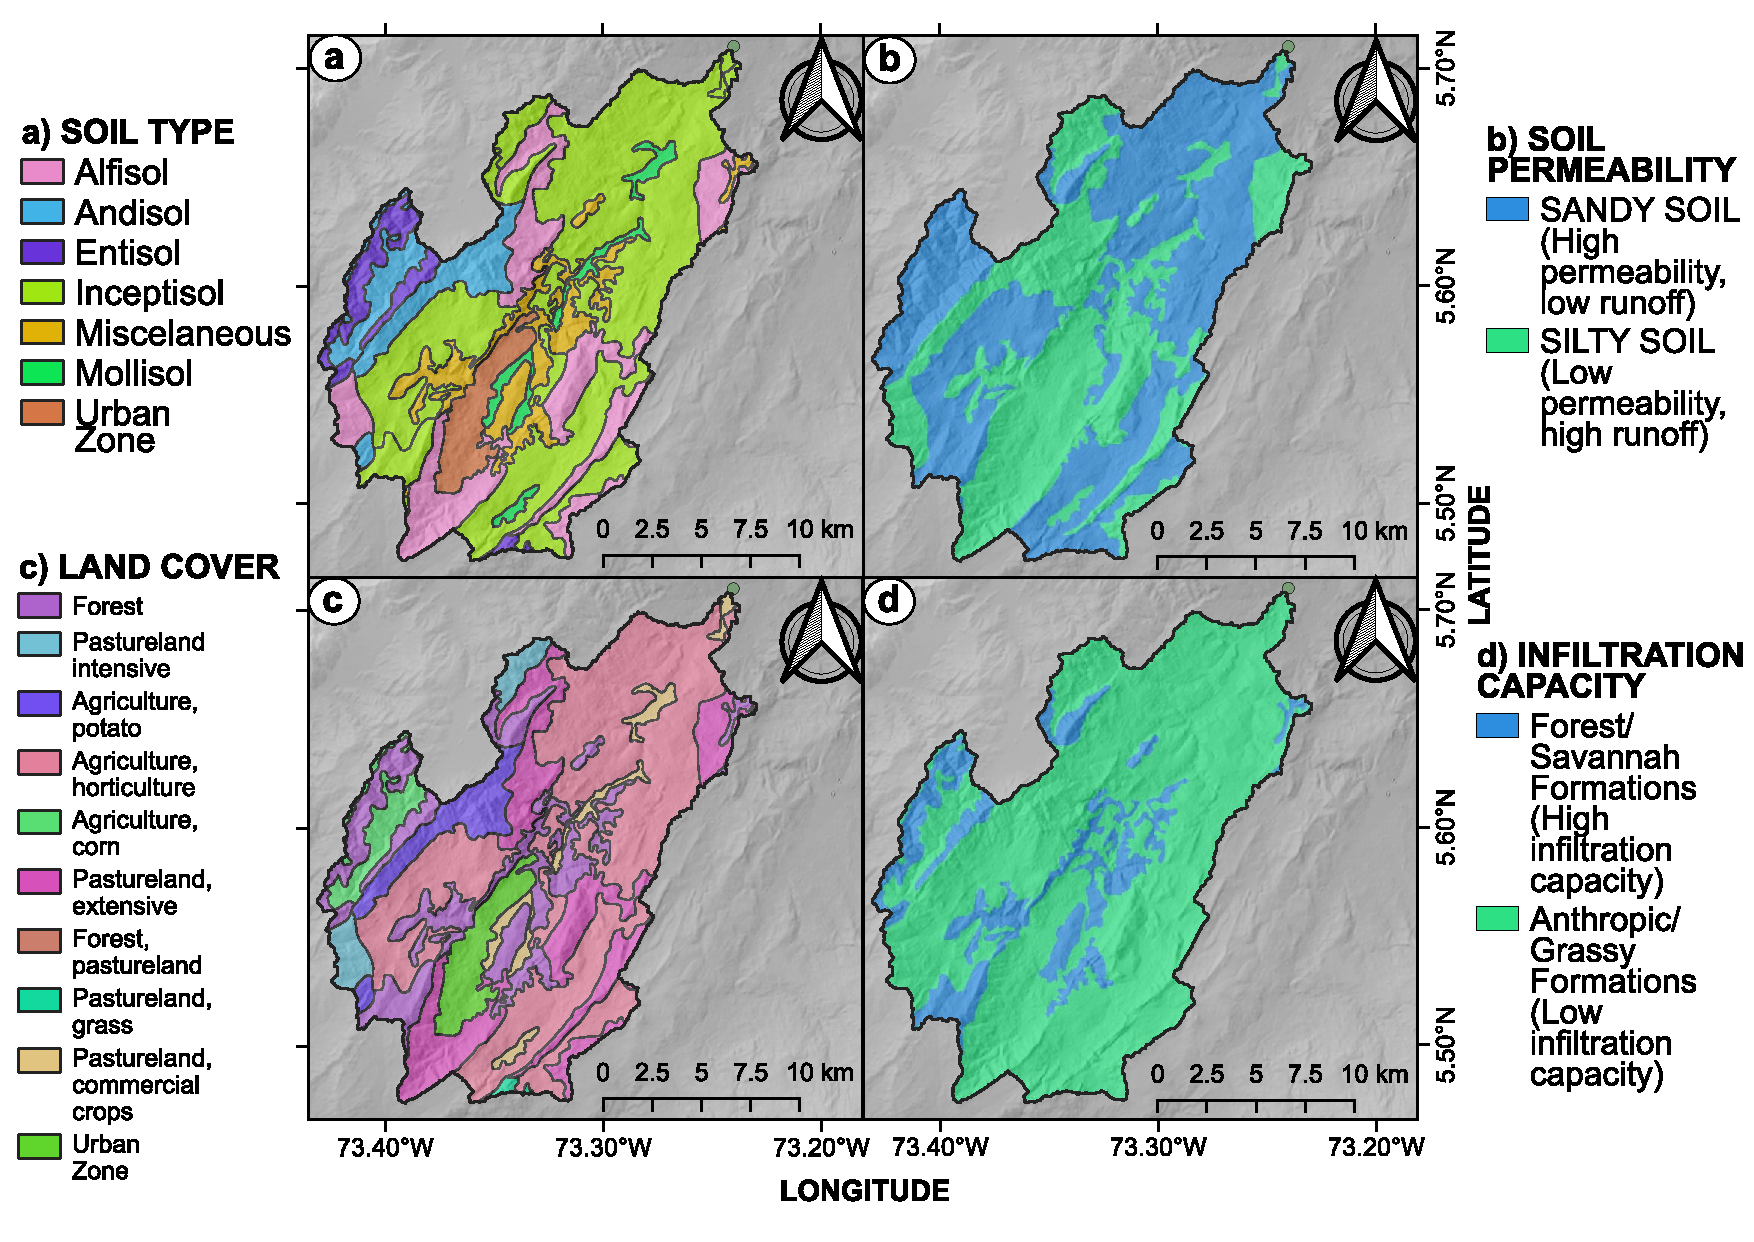
\includegraphics[scale=0.5]{Soil_variables1_Optimized.pdf}
	\caption{Soil information. a) Soil type. b) Soil permeability, c) Land use and land cover, d) Infiltration capacity.}\label{fig:soil}
\end{figure}

\subsubsection{Topographical Variables}
A DEM with a resolution of \SI{30}{\meter} is used to calculate the slope and reclassify these values in three different categories (see Table NUMBER) as shown in  Figure \ref{fig:input_variables2}.  The flat, moderate and steep areas occupy PERCENTAGES of the study area which indicates a rugged terrain. 

\begin{figure}
	\centering
	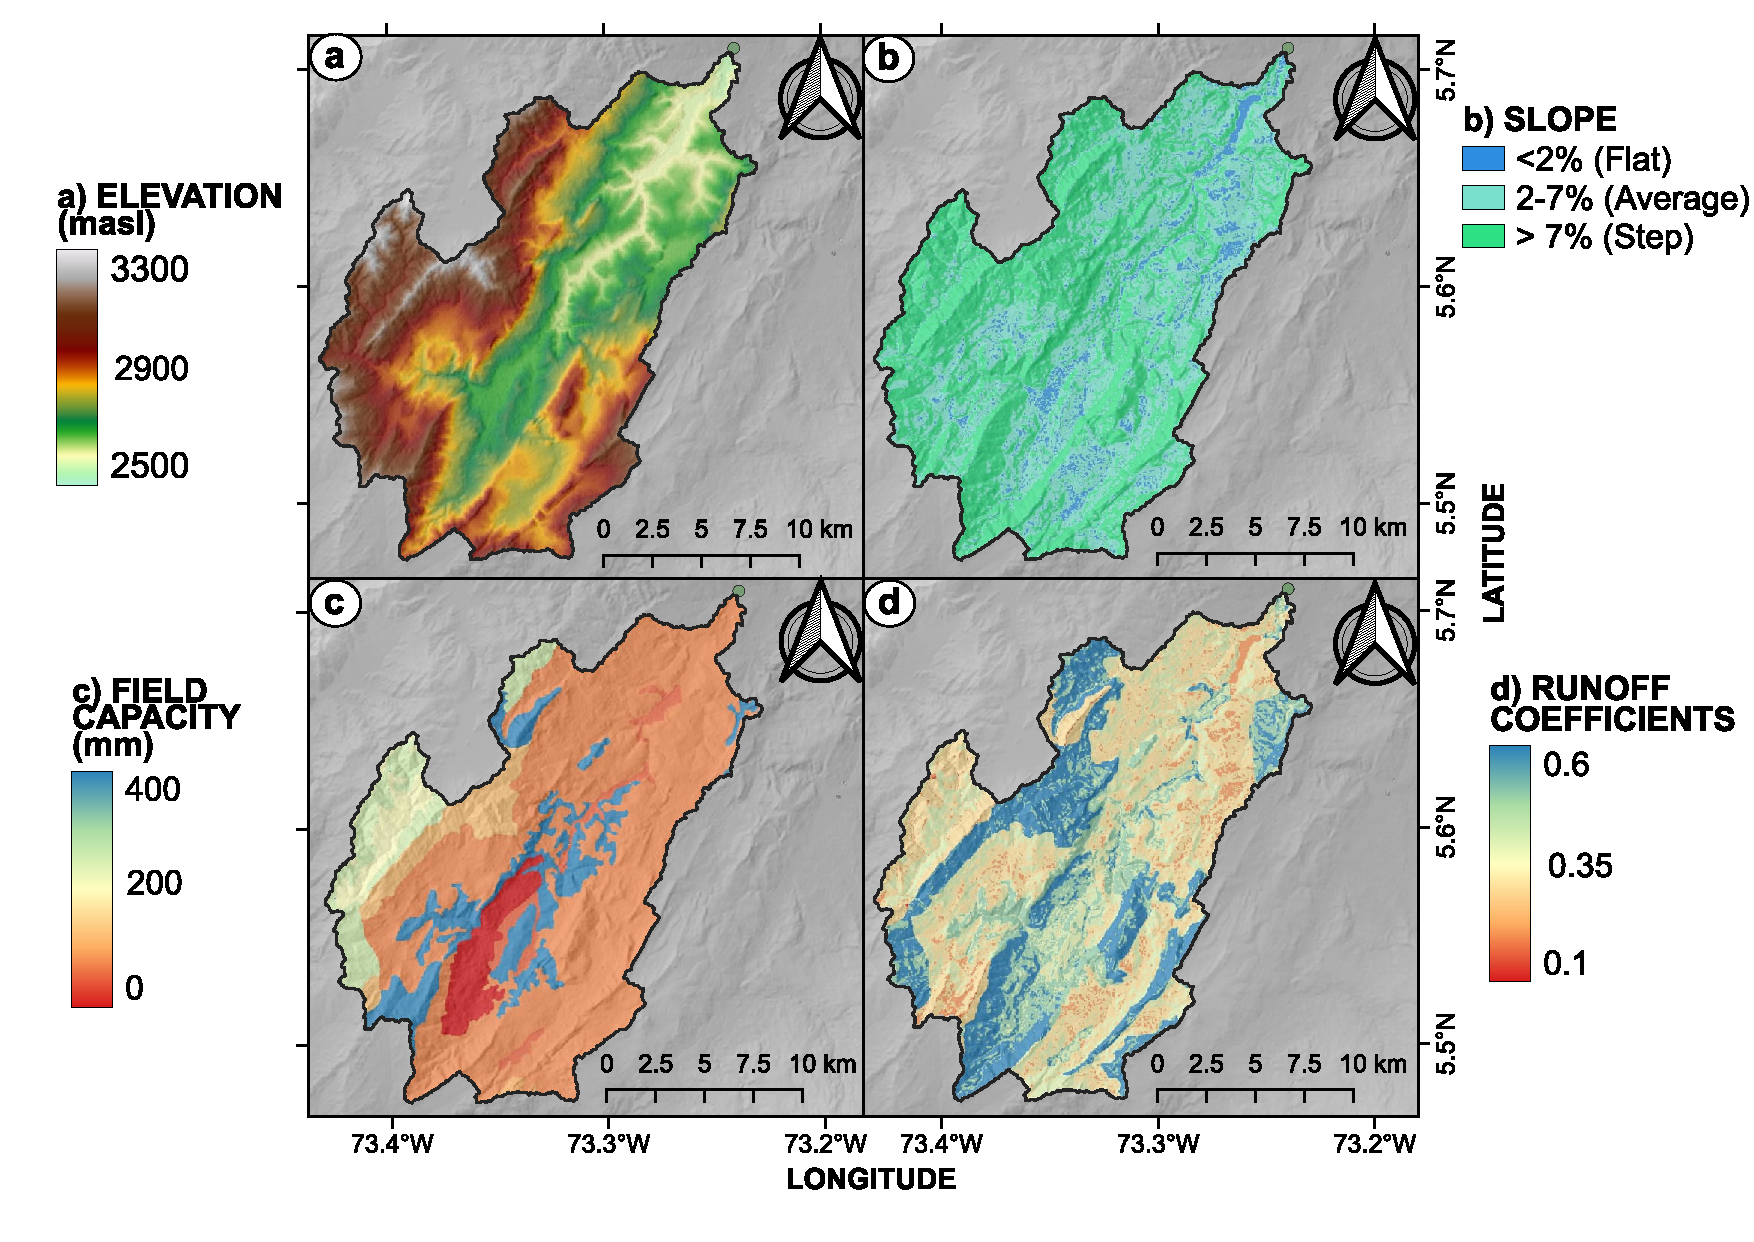
\includegraphics[scale=0.5]{Input_variables2_Optimized.pdf}
	\caption{Slope, Field Capacity and runoff coefficients.}\label{fig:input_variables2}
\end{figure}

\subsubsection{Field Capacity}

Figure \ref{fig:input_variables2}a shows the field capacity in the watershed defined from the soil type and land use and land cover using the values in Table \ref{tab:field_capacity}. The field capacity in most of the watershed has values close to \SI{100}{\milli \meter}, whereas the high values (\SI{400}{\milli \meter}) are located in scattered areas throughout the watershed. The minimum value of field capacity is located in the urban area of Tunja.

\begin{table}[!h]
	\centering
	\begin{tabular}{p{3cm}ccccc} \\ \hline
		& Sandy & Sandy loam & Silty loam & Clay loam & Silty \\ \hline
		Shallow rooted plants & 50 & 75 & 125 & 100 & 75 \\
		Moderately deep-rooted plants & 75& 150& 200& 200& 500 \\
		Deep-rooted plants & 100& 150& 250& 250& 200 \\
		Fruit& 150& 250& 300& 250& 300 \\
		Mature forest& 250& 300& 400& 400& 350 \\ \hline
	\end{tabular}
	\caption{Field capacity (mm) defined by soil type and use according to \cite{Thornthwaite1957}.}\label{tab:field_capacity}
\end{table}


\subsubsection{Runoff Coefficients}

Figure \ref{fig:input_variables2}d shows the runoff coefficients calculated combining the maps of soil permeability (Fig. \ref{fig:soil}b), infiltration capacity (Fig. \ref{fig:soil}d) and reclassified slope (Fig. \ref{fig:input_variables2}b) to define $12$ runoff classes. These classes are assigned the runoff coefficients shown in Table \ref{tab:runoff_classes}. The areas with low to intermediate values of runoff coefficients (0.1-0.3) are located in the NE, NW and SE parts of the study area whereas the high values (0.3-0.6) are mainly located in the SW part of the watershed.

\subsubsection{Hydrological Variables}
The mapping of hydrological variables has a problem related with the number of climatological and hydrological stations in the study area. There are only five hydrological stations and one climatological station and therefore it is not possible to obtain reliable maps of rainfall and temperature. The issue is solved by mapping the hydrological variables for the whole Boyaca state (see \label{fig:location}) with elevation as secondary variable. Let $Z(\boldsymbol{u},t_{i})$ be an random variable (rainfall or temperature in this case) measured at location $\boldsymbol{u}$ at the month $t_{i}$ that can be decomposed into: 
\begin{equation}
	Z(\boldsymbol{u},t_{i})=Z_{E}(\boldsymbol{u},t_{i})+R(\boldsymbol{u},t_{i}),t_{i}=1,\ldots,12
\end{equation}
where
\begin{itemize} 
\item $Z(\boldsymbol{u},t_{i})$ is the precipitation or temperature at location $\boldsymbol{u}=(x,y)$ and month $t_{i}$ 
\item $Z_{E}(\boldsymbol{u},t_{i})$ is the precipitation or temperature that depends on the elevation $h$
\begin{equation}
	P_{E}(\boldsymbol{u},t_{i})=m(t_{i})h+b(t_{i})
\end{equation} 
and $[m(t_{i}),b(t_{i})],t_{i}=1,\ldots,12$ are the slope and intercept of the linear regression model between precipitation/temperature and elevation for each month $i$.
\item $R(\boldsymbol{u},t_{i})$ is the residual component of $Z(\boldsymbol{u},t_{i})$ defined as 
\begin{equation}
R(\boldsymbol{u},t_{i})=Z(\boldsymbol{u},t_{i})-Z_{E}(\boldsymbol{u},t_{i})
\end{equation}
which is estimated over the whole state using: 
\begin{equation}
	R^{*}(\boldsymbol{u},t_{i})=\sum\limits_{j=1}^{N}\lambda_{j}R(\boldsymbol{u}_{j},t_{i})
\end{equation}
where the weights $\lambda_{j}$ can be obtained using ordinary kriging (OK) or inverse distance weighting (IDW). % __INCLUDE REFERENCES__
\end{itemize}

\paragraph{Precipitation}

The precipitation data is composed of monthly values of total rainfall measured at 107 hydrological stations between 1981-2020. These 29 years are classified in wet, normal and dry years with the SPI calculated using the following procedure:
\begin{itemize}
\item The total precipitation $TP_{i}$ is calculated for each year at each station between 1981-2020. 
\item The values of $TP_{i}$ are fitted to a Gamma distribution using Maximum Likelihood Estimation (MLE). 
\item The values of the Gamma CDF are calculated $$Z_{i}=F(TP_{i})$$
\item The values of $Z_{i}$ are transformed into a normal distribution $$SPI_{i}=y_{i}=G^{-1}\left[F(TP_{i})\right]$$These values of $SPI_{i}$ are used to classify each year into wet, normal and dry using the cutoffs in Table NUMBER.
\item A given year is  classified as wet, normal or dry according to the majority vote of the classification obtained for that year for all stations in the state.
\end{itemize}
%The monthly mean values of rainfall for wet, normal and dry years are calculated and these values are used to create the maps using the procedure previously explained as shown in Figure \ref{fig:precipitation}.   

Precipitation data for the watershed were extracted from monthly maps previously generated for the entire department, covering all water years in the study period. Figure \ref{fig:precipitation} compares monthly average rainfall patterns between summer and winter months (April and July, respectively) across these water years. In normal years, the watershed exhibits two distinct seasonal variations. During winter months (April), rainfall ranges between \qtyrange{30}{120}{\milli \meter}, with maximum values concentrated in the northeastern (NE) sector of the study area. In contrast, during summer months (July), precipitation decreases to \qtyrange{20}{70}{\milli \meter}, with higher values shifting to the eastern portions of the watershed. During dry years (Figs. \ref{fig:precipitation} b,c), precipitation shows reduced totals but similar spatial patterns.  In winter (April), rainfall varies in the \qtyrange{30}{100}{\milli \meter} range, where the high values are located towards the NE. In summer (July), rainfall decreases to \qtyrange{30}{60}{\milli \meter} range with peak values moving southeastward (SE). MISSING WET YEARS.

\begin{figure}
	\centering
	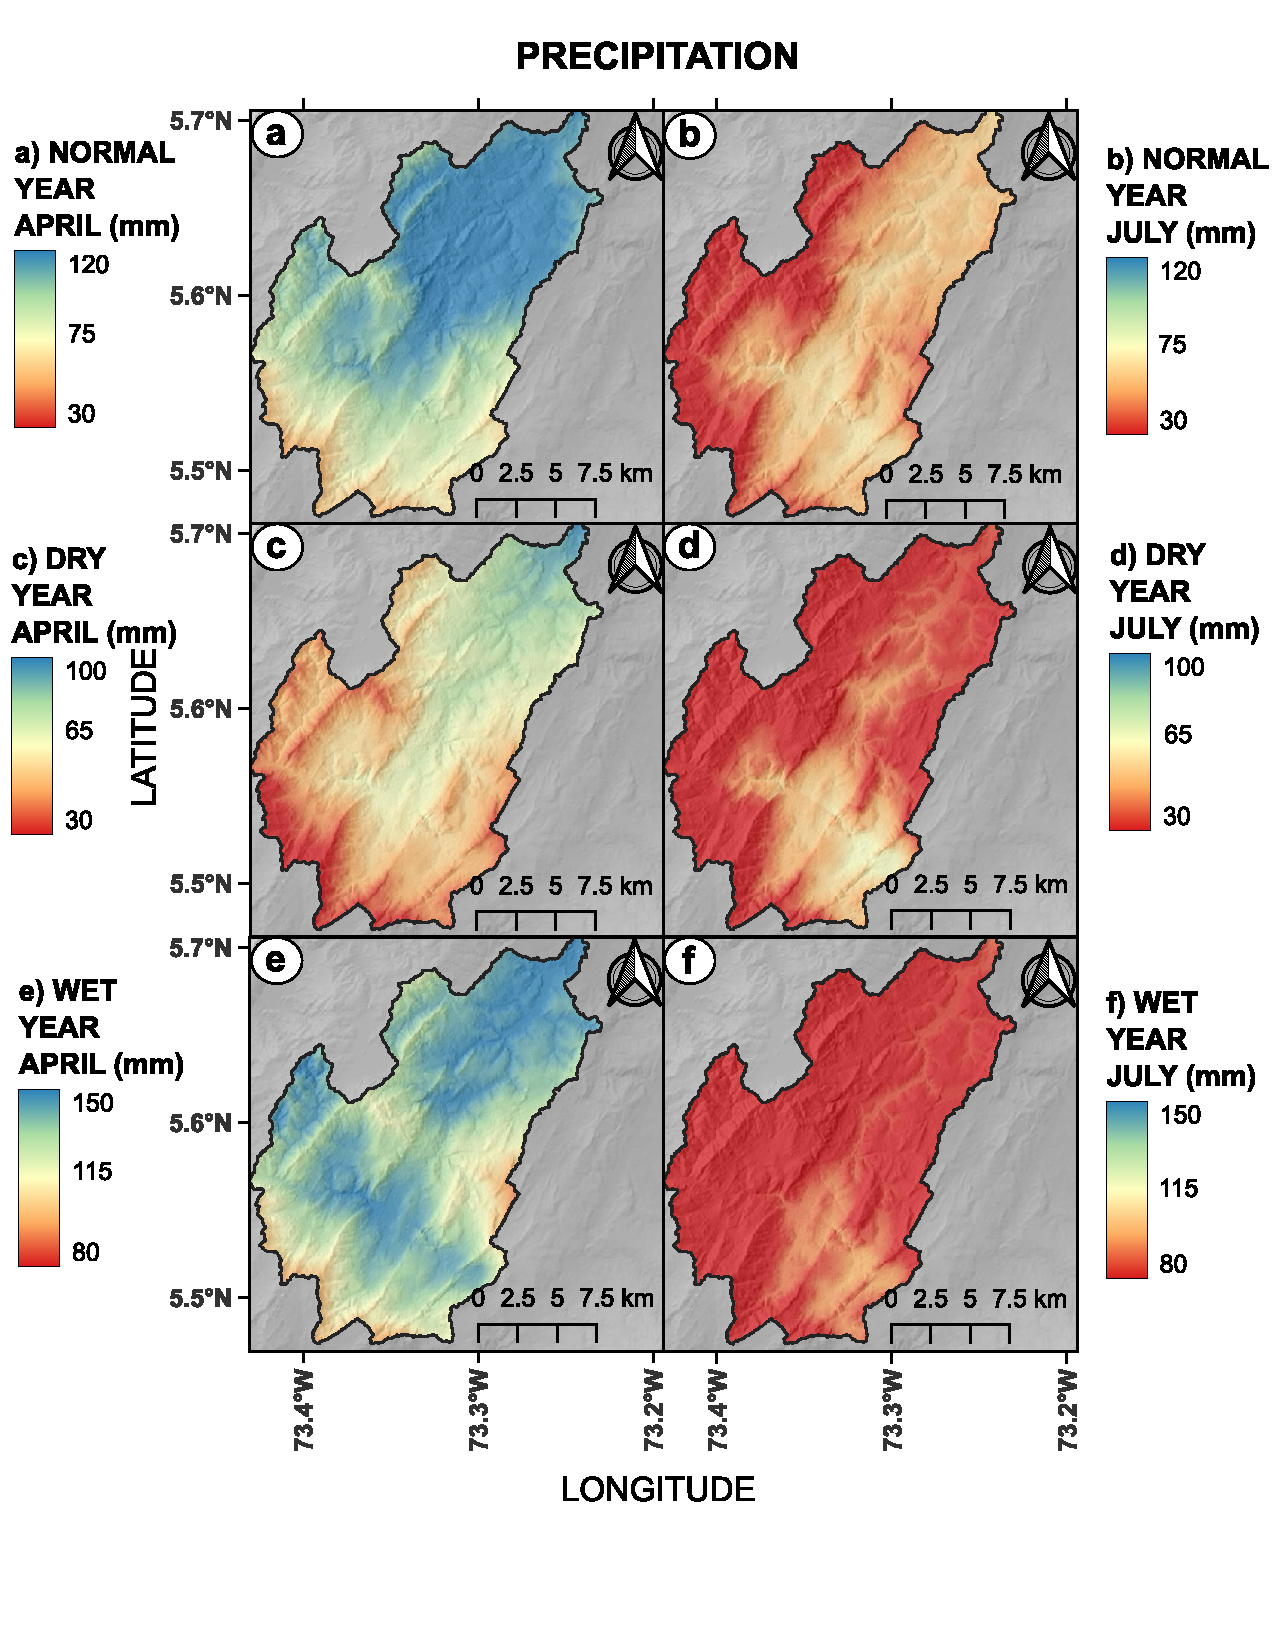
\includegraphics[scale=0.6]{precipitation1_Optimized.pdf}
	\caption{Precipitation}\label{fig:precipitation}
\end{figure}
	

\paragraph{Potential Evapotranspiration} Maps of monthly average temperature $T_{i}$ were generated for the Boyaca state for wet, normal and dry years using the procedure explained in eqs NUMBER to NUMBER with information from 28 climatological stations between 1981-2020 provided by IDEAM. The monthly temperature values had a weak dependence wrt elevation as shown by the correlation coefficients smaller than $0.5$ (see Table NUMBER). The residual component displayed no spatial correlation and therefore $R(\boldsymbol{u},t_{i})$ were interpolated by IDW with an exponent defined by cross-validation (see Table NUMBER). \\
\ \\
From these interpolated maps for the state. the values inside the Jordan River Watershed were clipped and used to  estimate the potential evapotranspiration using a modified Thornwaite approach explained in [[Koerner1997]], where a monthly heat index $I_{i}$ is calculated from $T_{i}$ in Celsius degrees using: 


\begin{equation}
I_{i}=(0.2T_{i})^{1.51} \;\text{For}\; T>0,i=1,\ldots,12
\end{equation}
The annual heat index $I_{y}$ is calculated as
\begin{equation}
	I_{y}=\sum\limits_{i=1}^{12}I_{i}
\end{equation}
The Unadjusted Potential Evapotranspiration UPET can be obtained using:
\begin{equation}
UPET=
\left\{
\begin{aligned}
	&0.53 \times \left(\frac{10T}{I_{y}}\right)^{\alpha},&\;\text{For}\; T < 27 \\
	&-0.015T^{2}+1.093T+14.208, &\;\text{For}\; T \ge 27
\end{aligned}
\right.
\end{equation}
where $\alpha$ is defined as:
\begin{equation}
\alpha=(6.75\times10^{-7})H_{y}^{3}-(6.75\times10^{-5})H_{y}^{2}+(0.01792)H_{y}+0.49239
\end{equation}
The Adjusted Potential Evapotranspiration APET can be calculated as the product between the mean sunlight duration for 12 h that depends on the latitude and month (see Table NUMBER) and UPET.

Table. Sunlight duration.

Figure NUMBER shows the APET calculated for different water years in the study area. There are small differences in the estimated APET for winter (April) and summer (July) for normal, dry and wet years. The high values of APET are located along the main line of Jordan river whereas the low values concentrate on the NW and SE parts of the study area.
\begin{figure}
	\centering
	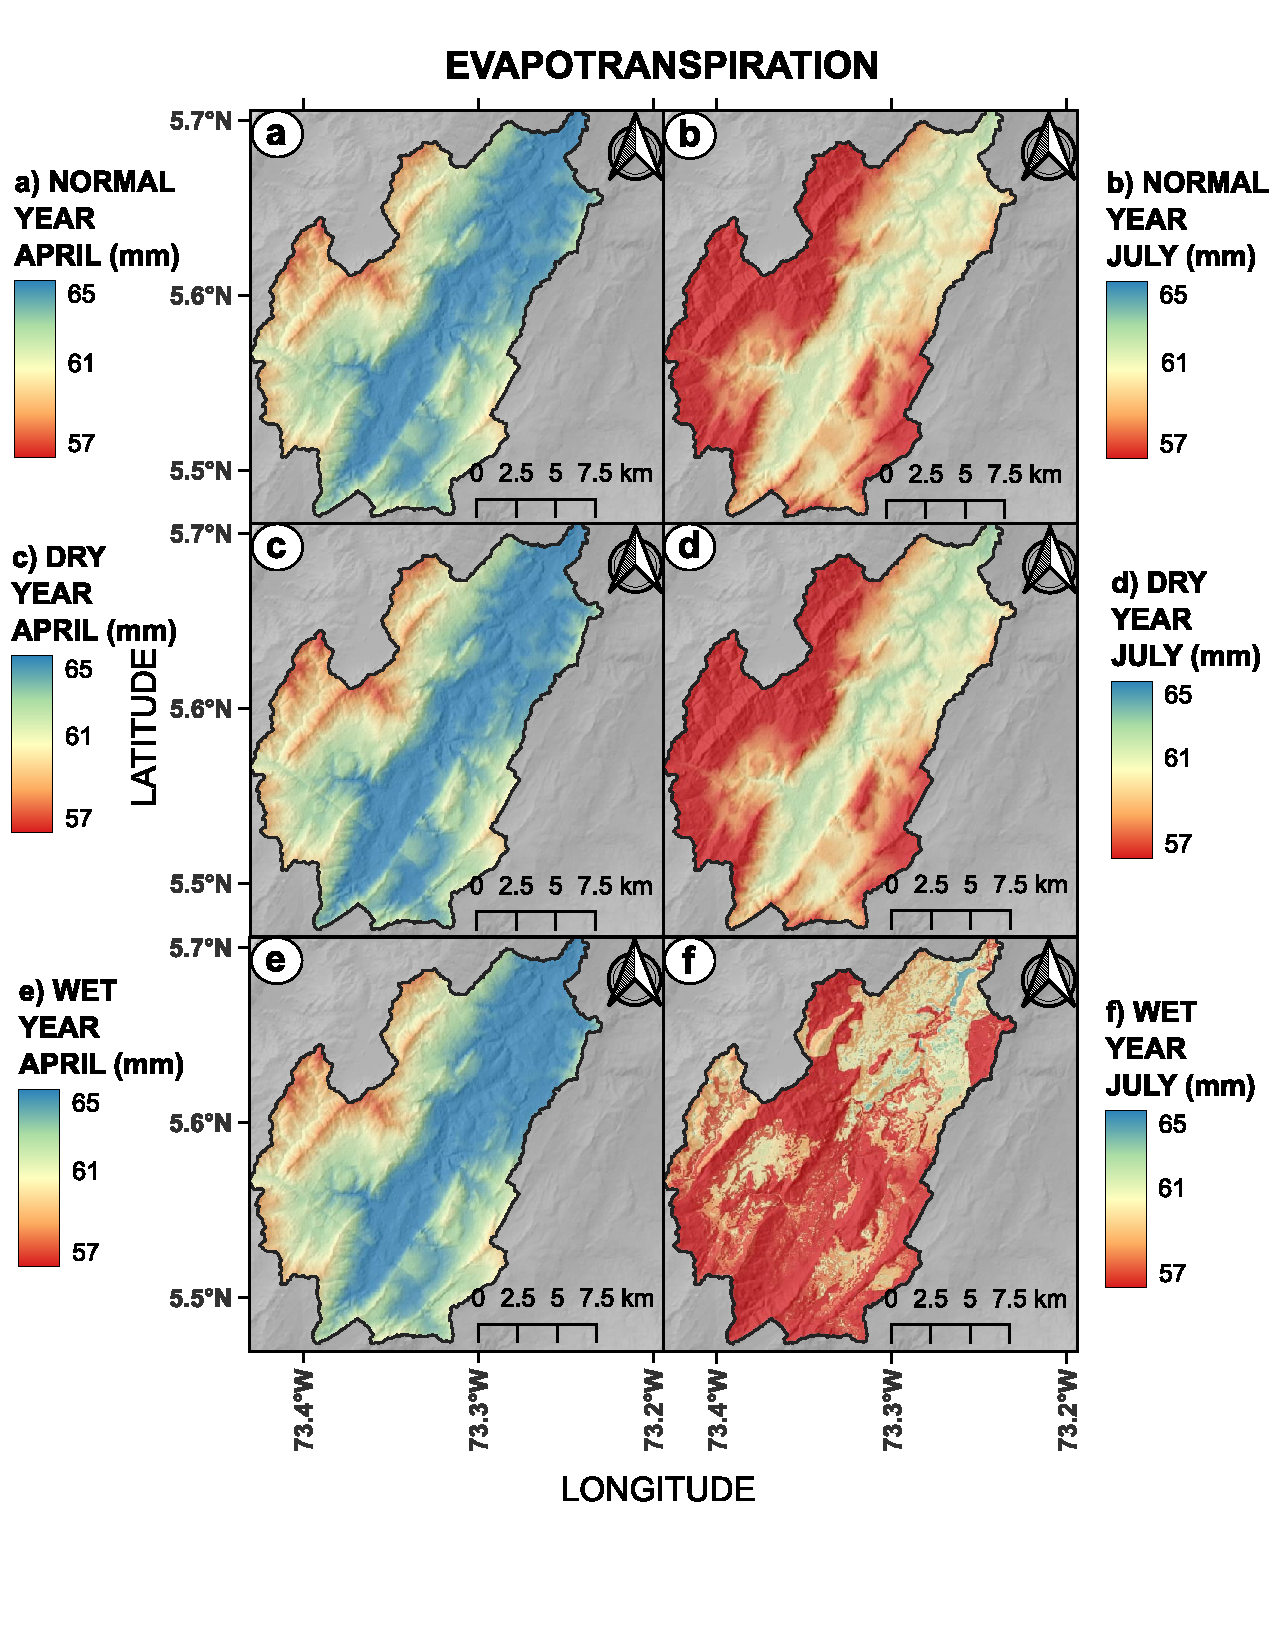
\includegraphics[scale=0.6]{evt_Optimized.pdf}
	\caption{Evapotranspiration}
\end{figure}

%%%%%%%%%%%%%%%%%%%%%%%%%%%%%%%%%%%%%%%%%%%
\section{Results and Discussion}

\subsection{General}

Figures \ref{fig:recharge_normal} and \ref{fig:recharge_wet}

Figure \ref{fig:recharge_annual} shows the results of the annual recharge estimated for the study area for normal, dry and wet years.  

\begin{figure}
	\centering
	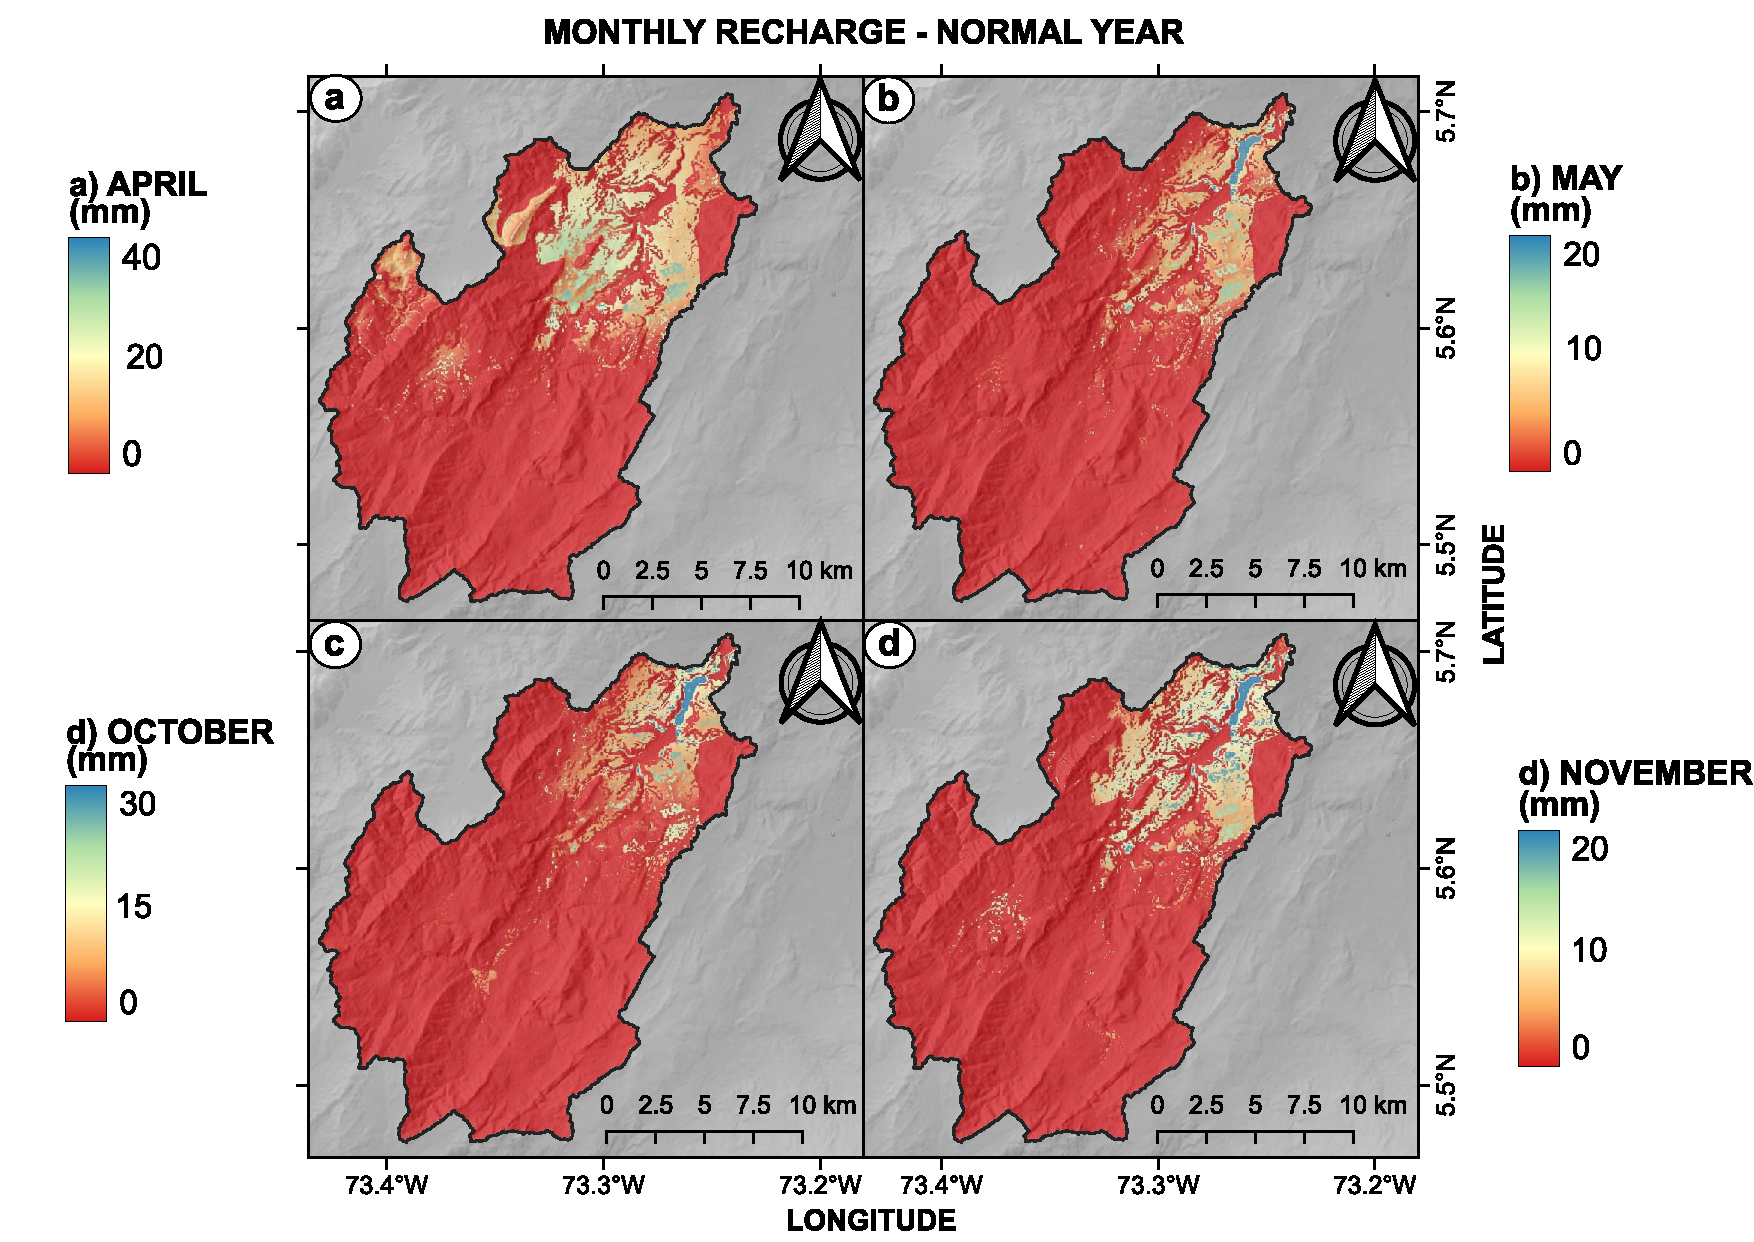
\includegraphics[scale=0.5]{montly_recharge_normal_Optimized.pdf}
	\caption{Monthly recharge normal year.}\label{fig:recharge_normal}
\end{figure}

\begin{figure}
	\centering
	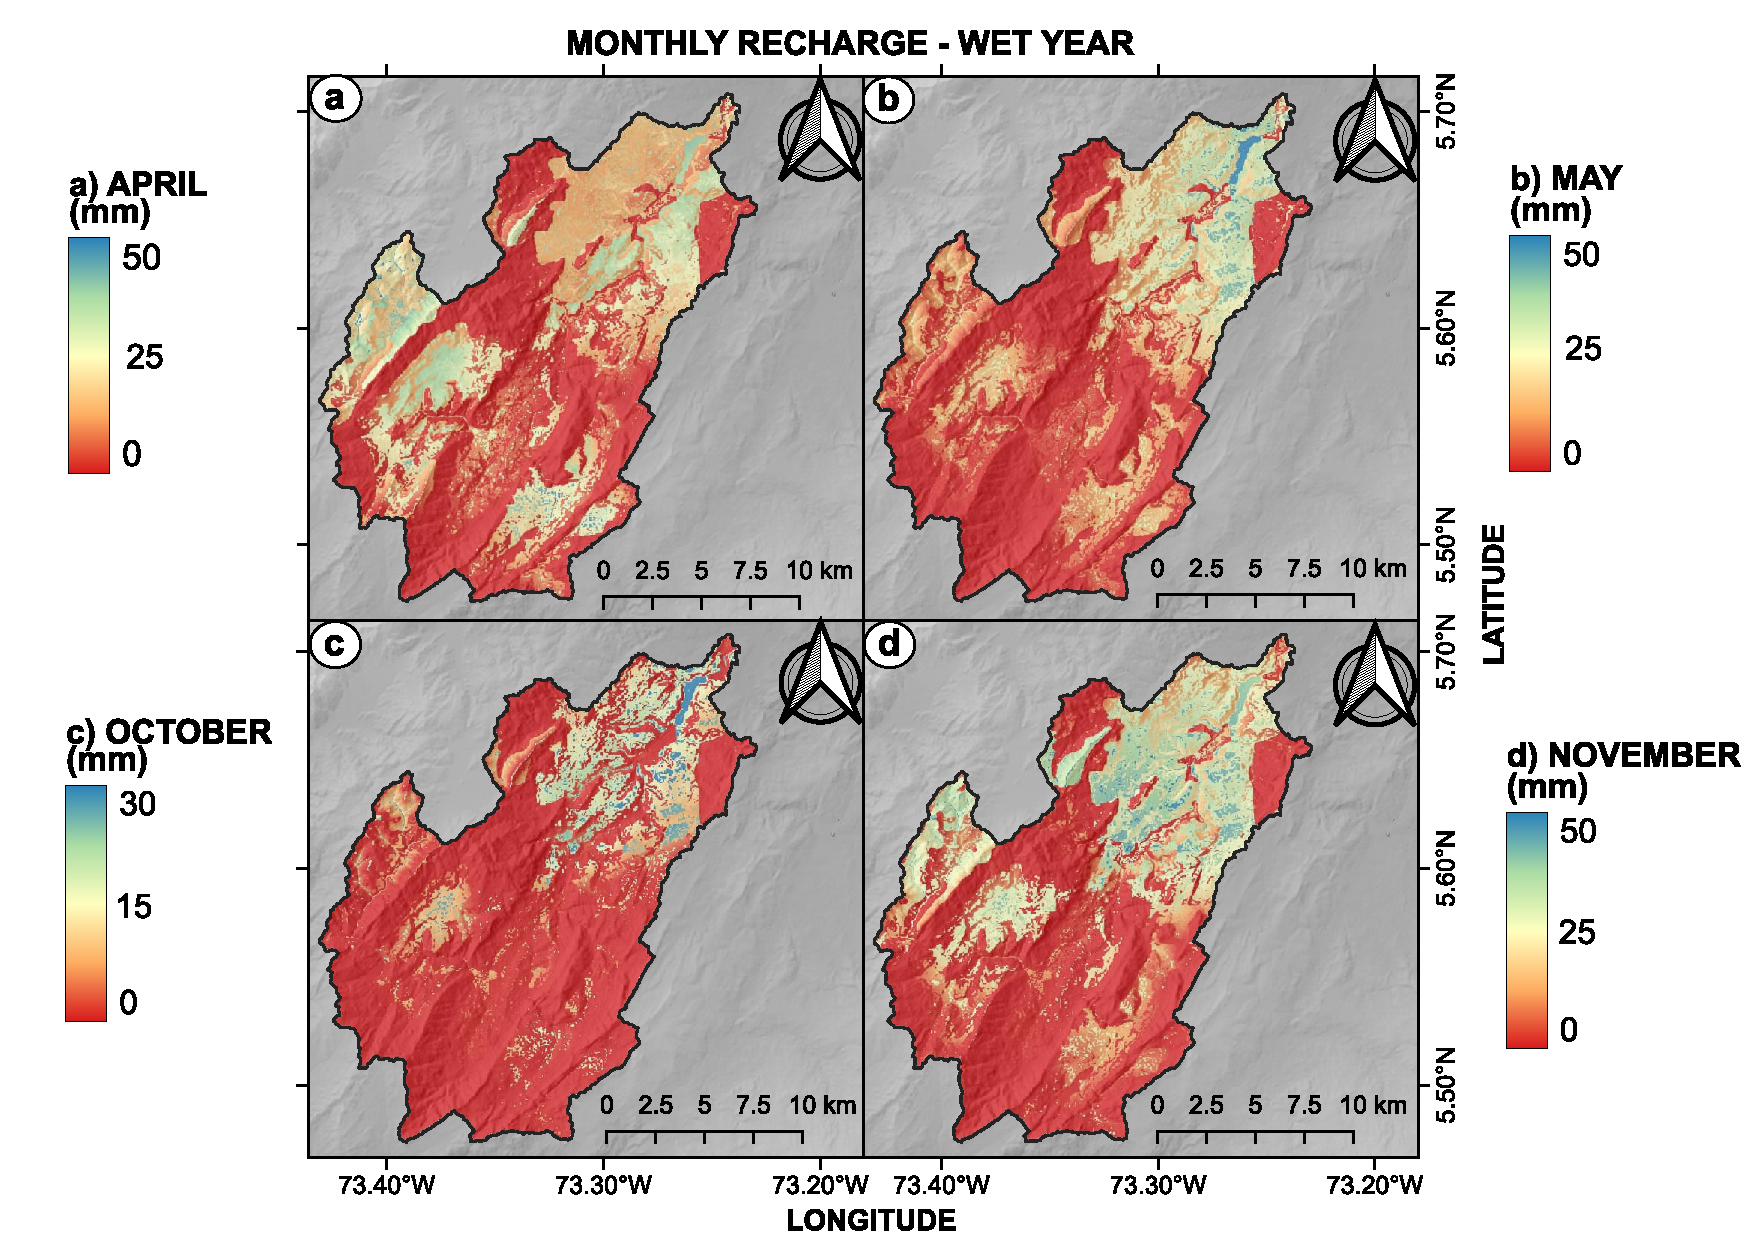
\includegraphics[scale=0.5]{montly_recharge_wet_Optimized.pdf}
	\caption{Monthly recharge wet year.}\label{fig:recharge_wet}
\end{figure}


\begin{figure}
	\centering
	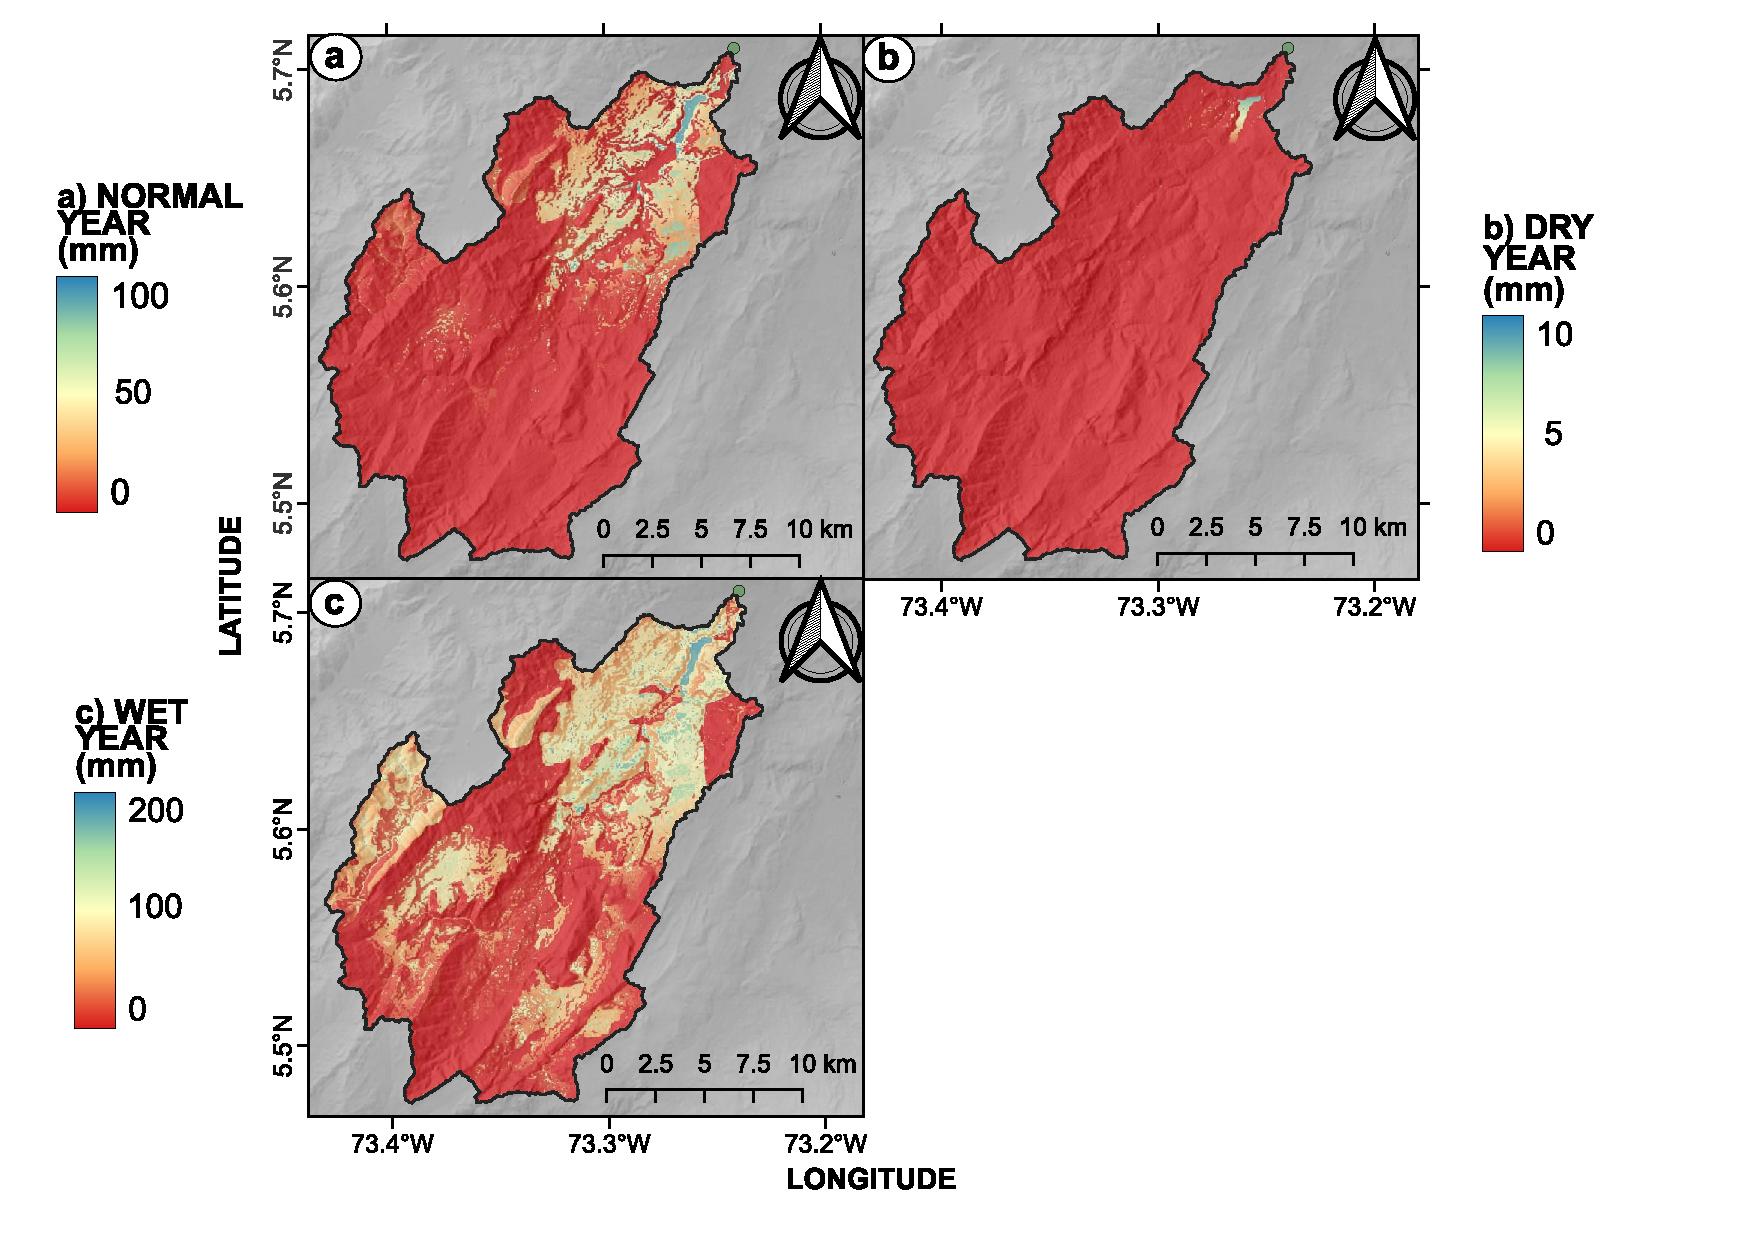
\includegraphics[scale=0.5]{recharge_Optimized.pdf}
	\caption{Annual recharge in the Vega River watershed obtained using the soil water balance approach. a) Annual recharge for a normal year, b) Annual recharge for a dry year, c) Annual recharge for a wet year. CALCULATE STATISTICS?. }\label{fig:recharge_annual}
\end{figure}


\subsection{Water balance by Runoff Classes}

\subsection{Water balance by Land Use Classes}

\subsection{Water Balance by Geological Unit}

%%%%%%%%%%%%%%%%%%%%%%%%%%%%%%
%\section{Discussion}
%
%\begin{itemize}
%	\item Answer Research Questions. Defend Answer with Results
%	\begin{itemize}
%		\item Q1: Magnitude (annual recharge). 
%		%Results shown in Figure \ref{fig:recharge_annual} indicate that groundwater recharge heavily depends  on the amount of precipitation over the study area. There is only \SI{10}{\milli \meter} of recharge to the aquifer in the north part of the study area during the dry years (see Fig. \ref{fig:recharge_annual}b), and there is no recharge in the aquifers located near the city of Tunja (SW part of the study area). 
%		%During a normal year, the annual recharge ranges between \qtyrange{50}{100}{\milli \meter} in the NE part of the study area in the Tilat� Fm and Quaternary deposits in Tuta municipality and in the Guaduas, Bogot� and Tital� Formations in Combita municipality, respectively.  The  annual recharge increases to \qtyrange{100}{200}{\milli \meter}.
%		
%		From the results, there are second recharge zones located in the study area. The first area called NE recharge area is located in the Tuta and Combita municipalities (see Fig. location) and it is characterized by annual recharges between \qtyrange{50}{100}{\milli \meter} during the normal years that increases to  \qtyrange{100}{200}{\milli \meter}  during wet years. The aquifers associated with this recharge zone include confined aquifers of the Tilata Fm and phreatic to locally confined aquifers in the Quaternary deposits.
%		
%		The second recharge area is located near Tunja municipality (capital of Boyaca state) and it is characterized by annual recharges between \qtyrange{20}{130}{\milli \meter} during the wet years with nill recharge during the dry and normal years. The aquifers associated with this recharge zones mainly include confined aquifers of the Bogota Formation.
%		
%		
%		
%		    
%		\item Q2: Places where recharge is high/low
%		\item Q3: Months where recharge is high. 
%	\end{itemize}
%	\item Explain
%	\begin{itemize}
%		\item Conflicting results
%		\item Unexpected findinds
%		\item Discrepancies with other research
%	\end{itemize}
%	\item Limitations
%	\item Importance
%	\item Newness
%\end{itemize}
%%%%%%%%%%%%%%%%%%%
\section{Conclusions}

%%===========================================================================================%%
%% If you are submitting to one of the Nature Portfolio journals, using the eJP submission   %%
%% system, please include the references within the manuscript file itself. You may do this  %%
%% by copying the reference list from your .bbl file, paste it into the main manuscript .tex %%
%% file, and delete the associated \verb+\bibliography+ commands.                            %%
%%===========================================================================================%%

\bibliographystyle{model3a-num-names}
\bibliography{GWRechargeRioJordan}% common bib file
%% if required, the content of .bbl file can be included here once bbl is generated
%%\input sn-article.bbl


\end{document}
